\section{Data Curation}

We construct two complementary Chinese image-text datasets for training and evaluating Chinese text-to-image models. The first is a general-purpose 9M Chinese image-text corpus, which is used to train the base Chinese text-to-image model and provides broad coverage of open-domain visual concepts, scene compositions, and natural-language descriptions. The second is a poem-grounded synthetic corpus containing 1,773,880 poem-image pairs, which is further used to adapt the base model to classical Chinese poetry-to-image generation. This two-stage data design allows the model to first acquire general Chinese text-to-image alignment and then specialize in the visual interpretation of classical poetry. The overall curation pipelines of the general Chinese text-to-image corpus and the poem-grounded corpus are illustrated in Fig.~\ref{fig:general_data_pipeline} and Fig.~\ref{fig:poem_data_pipeline}, respectively.

Compared with general natural-language prompts, classical Chinese poems pose additional challenges for text-to-image generation. Directly using original verses as generation prompts often leads to ambiguous or unstable synthesis results, owing to the condensed syntax, allusive expressions, and semantic distance between classical poetry and modern descriptive language. To address these challenges, we standardize the poetry corpus, convert poems into generation-oriented prompts, and pair the resulting prompts with synthesized images through a dedicated poem-grounded curation pipeline.

\begin{figure}[t]
\centering
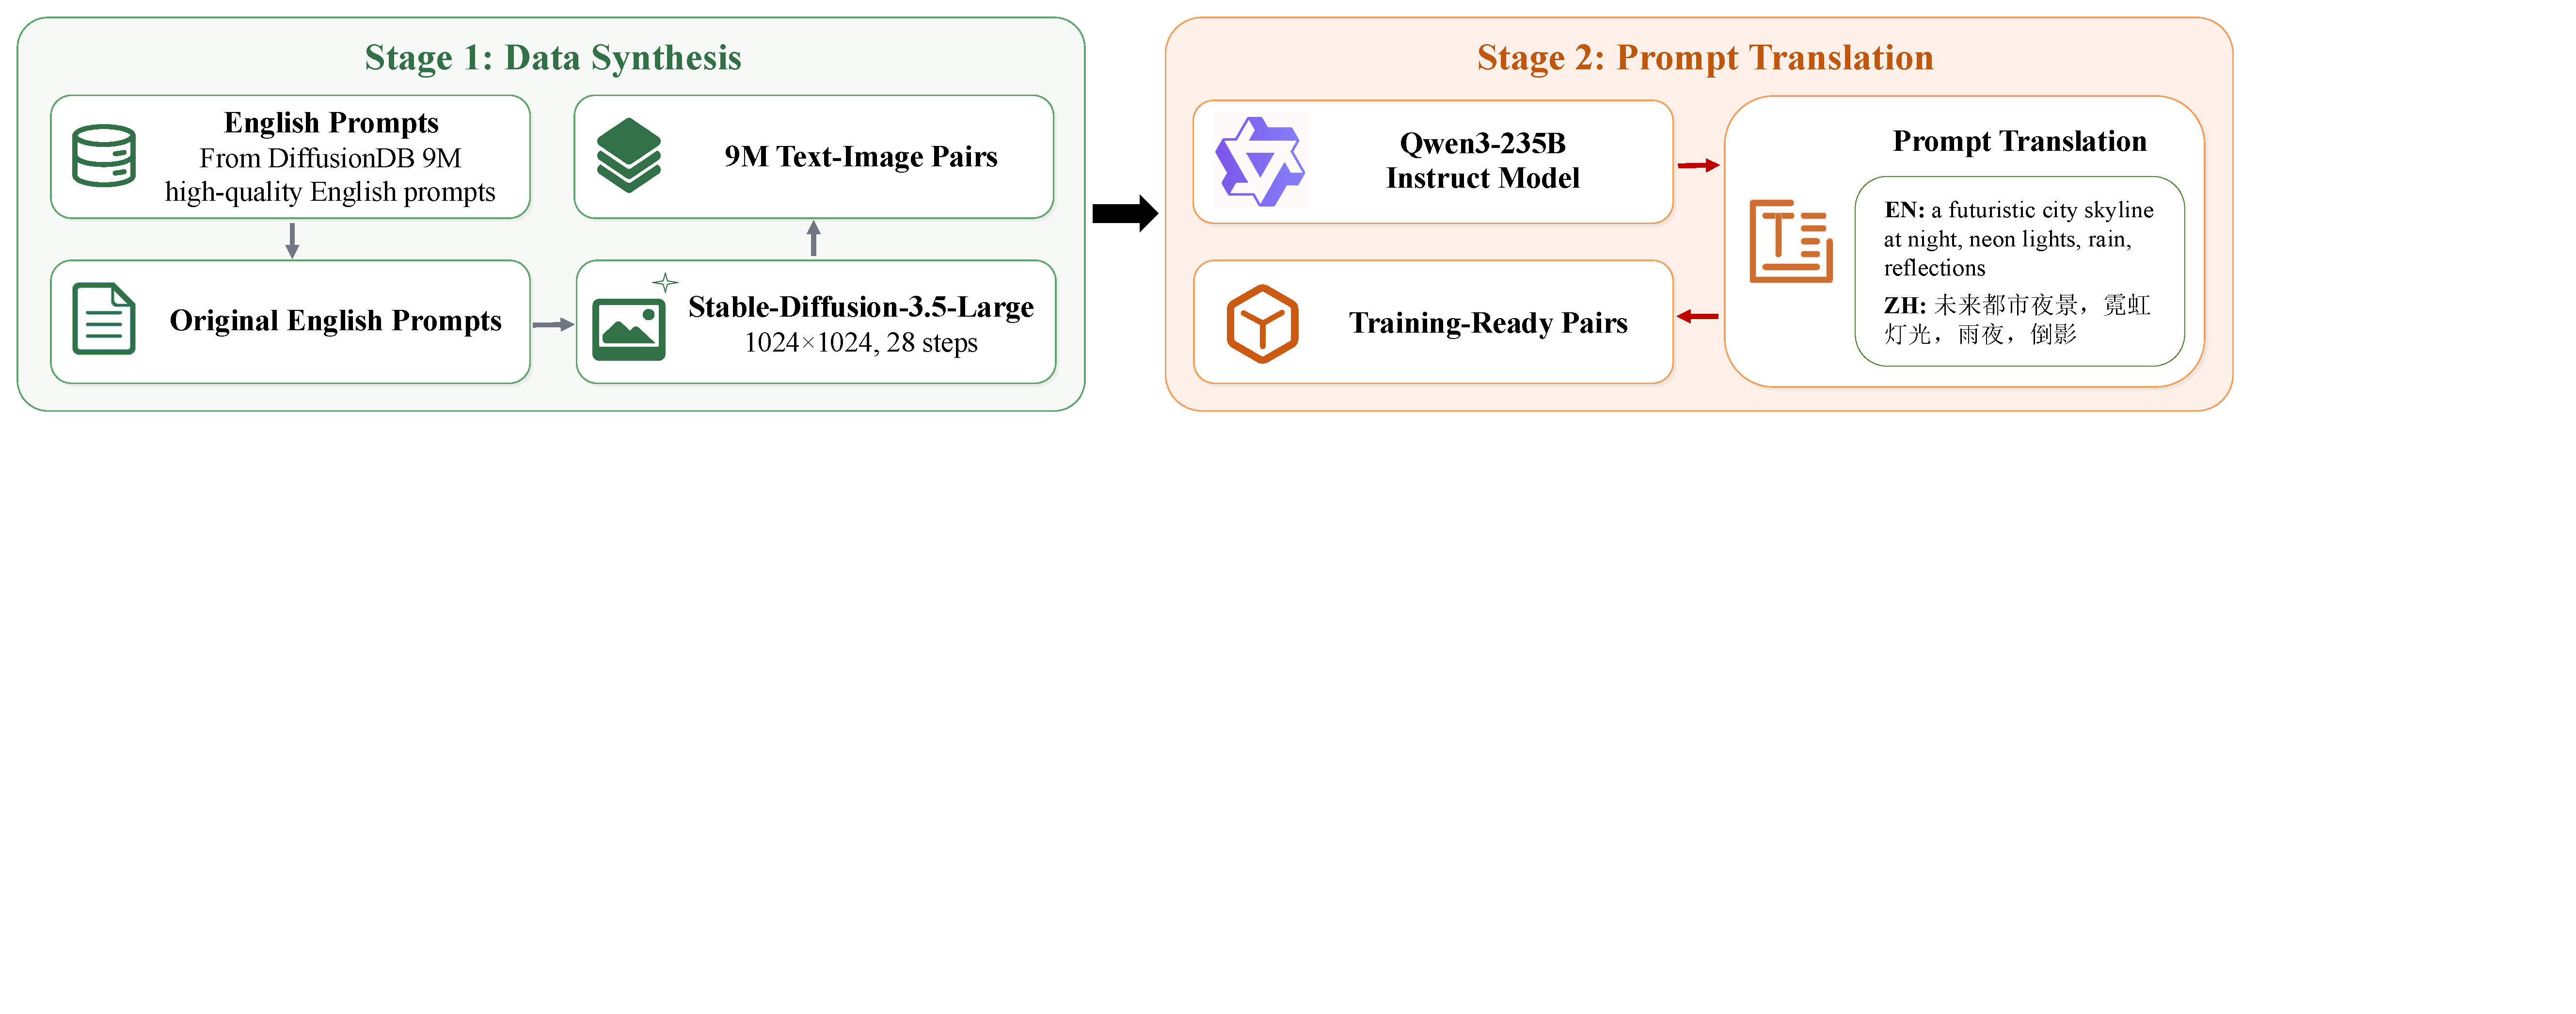
\includegraphics[width=\textwidth]{figures/figures/fig02.pdf}
%\caption{\textbf{Overview of the General Chinese Text-to-Image Curation Pipeline.}
%Two stages construct a 9M Chinese image-text corpus for training the Chinese text-to-image base model: 
%(1) Data Synthesis starts from 9M filtered English text-to-image prompts from DiffusionDB and uses the original English prompts to synthesize images via Stable Diffusion 3.5 Large; 
%(2) Prompt Translation converts the original English prompts into Chinese using Qwen3-235B-Instruct, producing training-ready Chinese prompt-image pairs while preserving the visual semantics of the original open-domain prompt distribution. }
\caption{\textbf{Overview of the General Chinese Text-to-Image Curation Pipeline.}
Two stages construct a Chinese image-text corpus for training the base model: 
(1) Data Synthesis starts from 9M filtered English text-to-image prompts from DiffusionDB and synthesize images via Stable Diffusion 3.5 Large; 
(2) Prompt Translation converts prompts into Chinese using Qwen3-235B-Instruct, producing training-ready Chinese prompt-image pairs. }
\label{fig:general_data_pipeline}
\end{figure}

\begin{figure}[t]
\centering
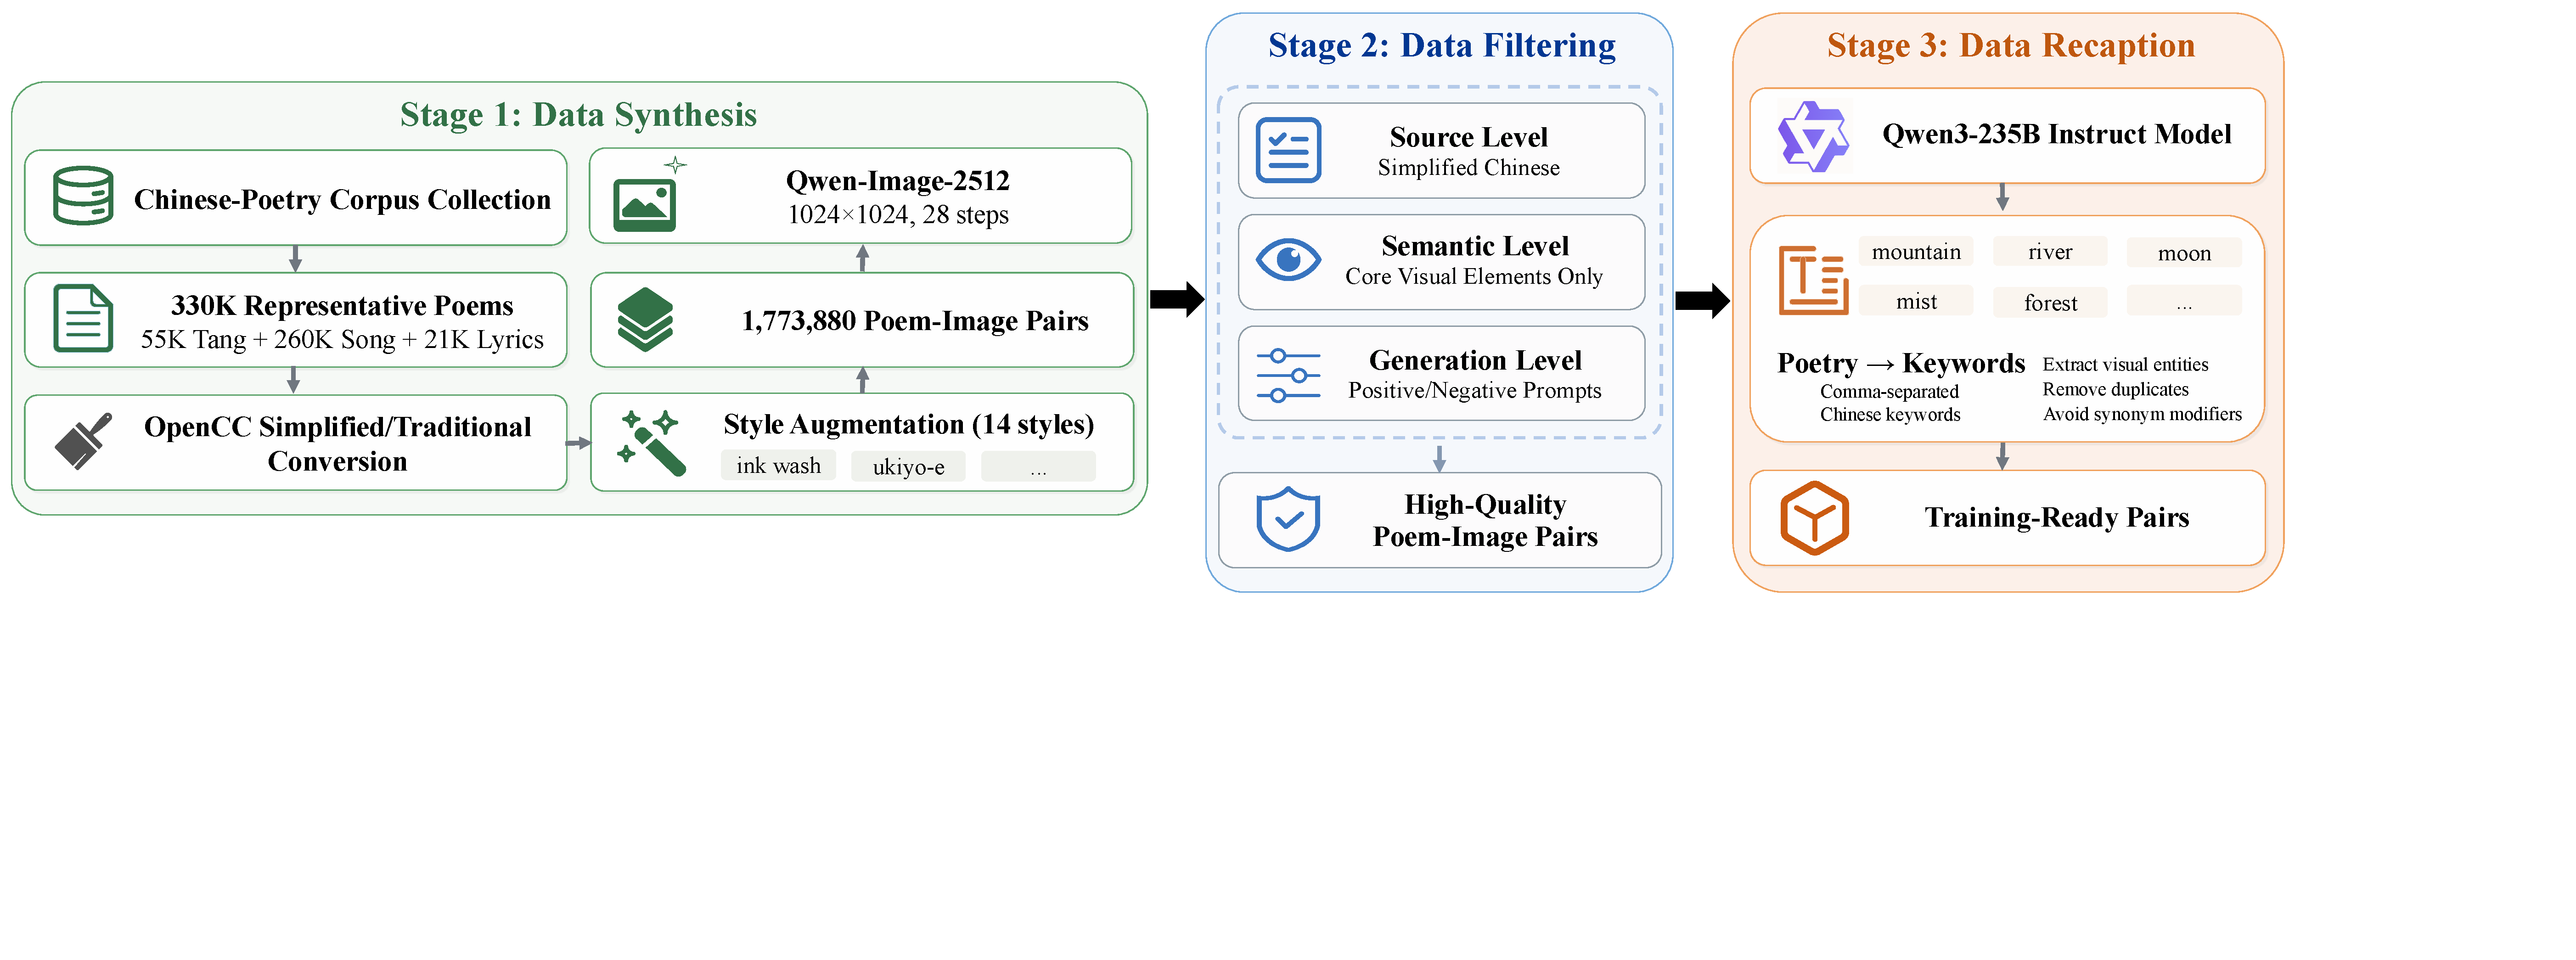
\includegraphics[width=\textwidth]{figures/figures/fig03.pdf}
\caption{\textbf{Overview of the Classical Poetry-to-Image Curation Pipeline.} Three stages transform classical Chinese poetry into 1,773,880 structured image-text pairs: (1)~Data Synthesis expands $\sim$330K poems with 14 stylistic descriptors and generates images via Qwen-Image-2512; (2)~Data Filtering applies source-level, semantic-level, and generation-level quality controls; (3)~Data Recaption converts each poem into compact keyword sequences via Qwen3-235B.}
\label{fig:poem_data_pipeline}
\end{figure}

% \subsection{Data Synthesis}

% We first construct a general-purpose 9M Chinese image-text corpus for base model training. Specifically, we start from a filtered set of 9M English text-to-image prompts derived from DiffusionDB~\cite{wang2022diffusiondb}. Each English prompt is used directly as the conditioning input to Stable Diffusion 3.5 Large to synthesize the corresponding image. After image generation, we translate the original English prompts into Chinese using Qwen3-235B-Instruct. The translated Chinese prompts are then paired with the generated images, forming a large-scale Chinese image-text corpus for general text-to-image pretraining. This construction strategy preserves the visual semantics of the original English prompt distribution during image synthesis while providing Chinese textual supervision for downstream model training.

% Based on the general Chinese text-to-image corpus, we further construct a poem-grounded dataset for classical Chinese poetry-to-image learning. We build the poetry corpus primarily from the public Chinese-Poetry repository~\cite{ChinesePoetry}, which contains large-scale collections of classical Chinese literature, including Tang poems, Song poems, Song lyrics, and other canonical texts. From this repository, we retain approximately 330,000 poems after removing duplicates, malformed entries, and non-poetic metadata. Since a substantial portion of the original materials is written in Traditional Chinese, we normalize the corpus into Simplified Chinese using OpenCC~\cite{BYVoidOpenCC} to ensure orthographic consistency for downstream processing and model training.

% To enrich the expressive diversity of the poem-grounded dataset, we further augment the poems with a broad set of stylistic descriptors. These descriptors span traditional East Asian visual styles, Western art movements, modern illustration styles, and speculative visual genres. This augmentation strategy expands the visual distribution of the generated data while keeping the original poem as the primary semantic anchor.

% After prompt construction, we synthesize poem-conditioned images using the open-source Qwen-Image-2512~\cite{wu2025qwenimagetechnicalreport} model. All images are generated at a resolution of $1024 \times 1024$ with 28 denoising steps. Each poem is paired with a subset of style-conditioned prompts after filtering, rather than exhaustively combined with all descriptors. Following this pipeline, we construct 1,773,880 poem-conditioned image-text pairs, which provide domain-specific multimodal data for poem-grounded image generation. 

\subsection{General Chinese Text-to-Image Corpus}

We first construct a general-purpose 9M Chinese image-text corpus for base model training. Specifically, we start from a filtered set of 9M English text-to-image prompts derived from DiffusionDB~\cite{wang2022diffusiondb}. Each English prompt is used directly as the conditioning input to Stable Diffusion 3.5 Large to synthesize the corresponding image. After image generation, we translate the original English prompts into Chinese using Qwen3-235B-Instruct. The translated Chinese prompts are then paired with the generated images, forming a large-scale Chinese image-text corpus for general Chinese text-to-image pretraining. 

This construction strategy avoids translation-induced prompt drift before image synthesis. Since the images are generated from the original English prompts, the visual semantics and open-domain distribution of the source prompt set are preserved. Meanwhile, the translated Chinese prompts provide Chinese textual supervision, enabling the model to learn general Chinese text-to-image alignment.

\subsection{Poem-Grounded Data Synthesis}

Based on the general Chinese text-to-image corpus, we further construct a poem-grounded dataset for classical Chinese poetry-to-image learning. We build the poetry corpus primarily from the public Chinese-Poetry repository~\cite{ChinesePoetry}, which contains large-scale collections of classical Chinese literature, including Tang poems, Song poems, Song lyrics, and other canonical texts. 
% From this repository, we retain approximately 330,000 poems after removing duplicates, malformed entries, and non-poetic metadata. Since a substantial portion of the original materials is written in Traditional Chinese, we normalize the corpus into Simplified Chinese using OpenCC~\cite{BYVoidOpenCC} to ensure orthographic consistency for downstream processing and model training.
From this repository, we retain approximately 330,000 poems after removing duplicates, malformed entries, and non-poetic metadata, and normalize the remaining corpus into Simplified Chinese using OpenCC~\cite{BYVoidOpenCC} to ensure orthographic consistency for downstream processing and model training.

To enrich the expressive diversity of the poem-grounded dataset, we further augment the poems with a broad set of stylistic descriptors. These descriptors span traditional East Asian visual styles, Western art movements, modern illustration styles, and speculative visual genres. This augmentation strategy expands the visual distribution of the generated data while keeping the original poem as the primary semantic anchor.

% The 14 stylistic descriptors define a candidate augmentation pool rather than an exhaustive Cartesian product. If fully expanded, $\sim$330K poems and 14 descriptors would yield approximately 4.6M candidates; after filtering, only a subset of valid poem-style combinations is retained, resulting in 1,773,880 poem-image pairs, or about 5.4 retained pairs per poem on average.
The 14 stylistic descriptors form a candidate augmentation pool rather than an exhaustive Cartesian product. A full expansion of approximately 330,000 poems across all 14 styles would produce about 4.6 million candidate combinations. We instead retain only poem--style pairs that pass the filtering process, yielding 1,773,880 poem--image pairs, corresponding to an average of approximately 5.4 valid style-conditioned images per poem.

After prompt construction, we synthesize poem-conditioned images using the open-source Qwen-Image-2512~\cite{wu2025qwenimagetechnicalreport}. All images are generated at a resolution of $1024 \times 1024$ with 28 denoising steps. Each poem is paired with a subset of style-conditioned prompts after filtering, rather than being exhaustively combined with all descriptors. Following this pipeline, we construct 1,773,880 poem-conditioned image-text pairs, which provide domain-specific multimodal data for poem-grounded image generation.

\subsection{Prompt Filtering and Quality Control}

The two datasets follow different prompt-processing strategies according to their roles in training. For the general 9M Chinese image-text corpus, we preserve the original English prompt semantics during image synthesis. Specifically, the filtered DiffusionDB prompts are used directly to condition Stable Diffusion 3.5 Large, without additional semantic pruning, style augmentation, or positive/negative prompt modification. The Chinese prompts are produced only after image generation through translation. This design avoids introducing translation-induced prompt drift before synthesis and maintains the broad open-domain distribution of the original prompt set for base model training.

% For the poem-grounded dataset, the filtering pipeline follows the three levels shown in Fig.~\ref{fig:poem_data_pipeline}. Source-level filtering standardizes the poetry corpus by removing duplicates, malformed entries, and non-poetic metadata, followed by Simplified/Traditional Chinese normalization with OpenCC. Semantic-level filtering restricts the recaptioned content to visually grounded entities and scene elements, removing repeated items and suppressing near-synonymous modifiers. Generation-level filtering regulates image synthesis through positive and negative prompt design, encouraging clear composition and high-resolution rendering while suppressing common visual artifacts.
For the poem-grounded dataset, we adopt the three-stage filtering pipeline illustrated in Fig.~\ref{fig:poem_data_pipeline}. At the source level, we clean and standardize the poetry corpus by removing duplicate poems, malformed entries, and non-poetic metadata, and then normalize Traditional Chinese text into Simplified Chinese using OpenCC. At the semantic level, we retain only visually grounded entities, objects, and scene descriptions from the recaptioned content, while eliminating redundant elements and near-synonymous modifiers. At the generation level, we incorporate carefully designed positive and negative prompts to promote high-resolution rendering and coherent composition while mitigating common visual artifacts.

At the image generation stage for the poem-grounded dataset, we further regulate output quality through positive and negative prompt design, following common practices in large-scale text-to-image generation and data construction~\cite{schuhmann2022laion,wang2022diffusiondb,openclip2022,zhang2024longclip}. The positive prompt encourages desirable visual attributes such as high-resolution rendering, clear composition, and cinematic visual quality. In parallel, the negative prompt suppresses common generation artifacts, including low-resolution images, texture defects, anatomical distortions, oversaturation, unnatural facial appearance, blurred or distorted text, and visually disordered layouts. Rather than relying on an additional post-hoc classifier or filtering module, these controls are integrated directly into the prompt construction and generation process. They serve as a lightweight mechanism for encouraging higher visual quality and reducing visually implausible outputs during large-scale poem-grounded dataset construction.

\subsection{Data Recaption}

The recaptioning stage reformulates each source poem into a compact, visually grounded keyword sequence suitable for Chinese text-to-image generation. This step is necessary because classical Chinese poetry often encodes scenery, objects, emotions, and historical allusions in a highly condensed literary form, whereas modern text-to-image models typically require explicit and visually grounded prompts. To bridge this gap, we employ Qwen3-235B-A22B-Instruct-2507~\cite{qwen3technicalreport} to convert each poem into a comma-separated list of Chinese keywords compatible with diffusion-based text-to-image prompting.

The recaptioning process operationalizes the semantic pruning constraints described above through a constrained instruction format. Rather than performing literal translation, the model maps the condensed literary expression of each poem into explicit visual elements and standardized prompt tokens. The instruction asks the model to extract core realistic visual elements, retain a compact keyword or phrase for each salient object or scene component, remove repeated descriptions, avoid synonymous stacking, and output concise Chinese keywords separated by commas. As a result, the generated prompts are compact, non-repetitive, visually grounded, and can be directly used as inputs to downstream image generation models.

When a stylistic descriptor is appended to the source poem, the recaptioning model incorporates the corresponding style token into the generated prompt while keeping the extracted scene elements unchanged. This enables style-conditioned generation using a unified prompt format. For example, a poem describing a ruined palace site and flowing water can be reformulated into visual keywords such as “palace ruins, millet seedlings, ruined terrace, deer, fresh grass, river, white waves”. When the poem is associated with a specific artistic style, the corresponding style token is appended to the extracted scene elements.

Overall, the resulting corpus is organized as poem-prompt-image triplets. In each triplet, the original poem provides the literary source, the recaptioned prompt provides a standardized generation-oriented textual representation, and the synthesized image provides the corresponding visual realization. These triplets provide structured text-image supervision for poem-grounded image generation and related downstream multimodal learning~\cite{liu2023bdm,chinese-clip}.

\subsection{Edge-Oriented Prompt Refiner Supervision}

While the teacher-generated prompts described above are effective for large-scale dataset construction, our deployed Android application must handle raw classical poems directly provided by users. This creates a deployment-time interface gap: the image generation model expects explicit and visually grounded prompts, whereas users naturally interact with the system through original poetic text. Therefore, beyond constructing poem-prompt-image triplets for image model training, we further reuse the raw poems and their teacher-generated prompts to build text-to-text supervision for an edge-oriented prompt refiner.

% Specifically, we use Qwen3-235B-A22B-Instruct-2507 as an offline teacher model to generate structured visual prompts from raw classical poems. Each training instance is organized as a raw-poem/teacher-generated-prompt pair, where the raw poem serves as the input sequence and the teacher-generated prompt serves as the target output. This formulation distills the teacher model's prompt-construction behavior into a supervised learning problem for a substantially smaller language model.
Specifically, we use Qwen3-235B-A22B-Instruct-2507 as an offline teacher model to generate structured visual prompts from raw classical poems. The teacher-generated prompts preserve the core poetic semantics while making implicit imagery more explicit and visually grounded. Each training instance is organized as a raw-poem/teacher-generated-prompt pair, where the raw poem serves as the input sequence and the teacher-generated prompt serves as the target output. This formulation distills the teacher model's prompt-construction behavior into a supervised learning problem for a substantially smaller language model.

Since Qwen3-235B-A22B-Instruct-2507 is impractical for mobile edge devices due to its prohibitive memory and computational requirements, we fine-tune Qwen3-1.7B using LoRA on the constructed raw-poem/teacher-generated-prompt pairs. The LoRA adaptation specializes the smaller model for poetry-oriented prompt refinement without requiring full-parameter fine-tuning. As a result, the adapted Qwen3-1.7B model learns to transform raw classical poems into generation-ready prompts that are better aligned with the downstream diffusion model.

In the final system, the fine-tuned Qwen3-1.7B model is deployed and executed on Android devices as an on-device prompt refiner. Given a user-provided poem, it first generates a refined visual prompt, which is then passed to the poetry-oriented text-to-image model for image synthesis. For Android deployment, the adapted model is optimized for mobile inference to reduce memory usage and latency. This design decouples offline large-model supervision from online edge inference: the 235B teacher model provides prompt supervision during data construction, while the LoRA-tuned~\cite{hu2024lora} 1.7B model enables practical on-device prompt refinement in the deployed Android application.